\section{实验}

\subsection{研究问题与协议}

我们回答四个问题：共识是否减少一阶许可？是否改善hard endpoint？是否产生超过scale source的非零状态？失败时部署与正式测试如何处理？模型为Meta-Llama-3.1-8B-Instruct，共同Vector-GSQ锚点使用4096条FineWeb-Edu train、128 validation、512 Vector-GPTQ序列，长度4096。任务适应开放layers 28--31；五项任务各使用512 train、256 validation、31 audit，audit offset为1088。文本为4096 train、128 validation、64 audit，长度4096，新audit rows为5504--5567。

训练固定两轮、seed 0，不扫描学习率、group size、候选数、视图数或投影比例。正式PPL协议为WikiText2 raw test、seqlength 2048；准确率为\texttt{lm\_eval 0.4.4}全量0-shot ARC-C/E、HellaSwag、LAMBADA、PIQA与WinoGrande。实验串行使用一张A100 80GB。

\subsection{Figure 1：共识漏斗与硬端点}

\begin{figure*}[t]
  \centering
  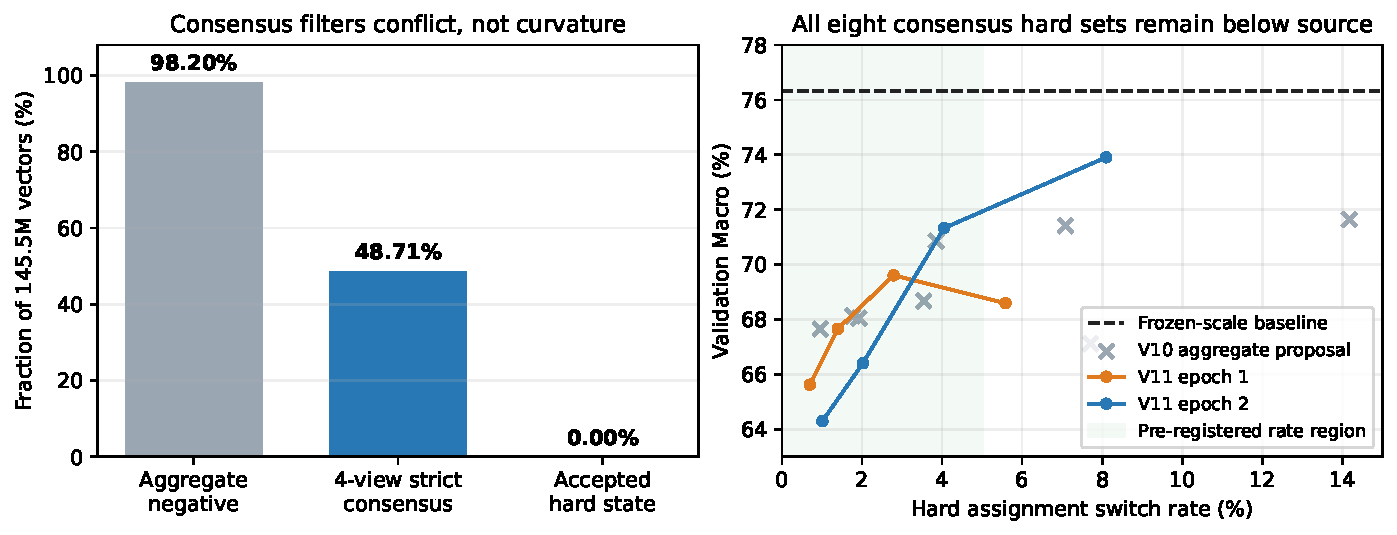
\includegraphics[width=0.98\textwidth]{../img/v11_consensus_gate.pdf}
  \caption{左：聚合负方向经四视图严格共识从98.20\%降至48.71\%，但最终接受率为0。右：V11改善最佳changed endpoint，八个共识硬集合仍全部低于冻结scale。}
  \label{fig:consensus}
\end{figure*}

Figure~\ref{fig:consensus}区分过滤有效与方法成功。候选池约减半说明梯度冲突存在，但零accepted hard state说明其不是充分解释。V11 epoch 2比V10更接近source，5\%预注册区域内仍无例外。

\subsection{同模型部署端点}

\begin{table*}[t]
\centering
\caption{同一Llama-3.1-8B-Instruct上的部署端点。QTIP不使用目标任务标签，仅用于通用PTQ质量定位。}
\begin{tabular}{lclrrr}
\toprule
端点 & 任务标签 & 主要变化 & PPL$\downarrow$ & Macro-6$\uparrow$ & 五任务$\uparrow$\\
\midrule
QTIP & 否 & 2.0-bpp trellis & \textbf{8.7971} & 69.8469 & 69.8749\\
Vector-GSQ anchor & 否 & 无 & 10.4960 & 67.9997 & 68.1046\\
Assignment-only & 是 & 0.3781\% index & 10.7347 & 69.4774 & 69.0744\\
Scale-only & 是 & 5.52M FP16 scale & 10.9448 & \textbf{71.7223} & \textbf{72.5484}\\
Naive joint & 是 & scale + 0.8610\% index & 11.4098 & 69.7434 & 68.9511\\
V10 aggregate handoff & 是 & 最终0 switch & 10.9448 & 71.7223 & 72.5484\\
V11 consensus handoff & 是 & 最终0 switch & 10.9448 & 71.7223 & 72.5484\\
\bottomrule
\end{tabular}
\label{tab:endpoints}
\end{table*}

V11不产生新Pareto endpoint。Assignment-only仍是PPL漂移较小的独立分支，但不再作为scale后续模块。由于监督不同，不能据任务平均声称公平超过QTIP。

\subsection{共识过滤量}

总计145,465,344个向量。聚合梯度负邻居率为98.1973\%，四视图加权严格共识率为48.7101\%；70,856,267个向量合格，74,609,077个精确冻结。28个Linear的共识率为37.4745\%--74.9129\%，选中邻居平均最差视图变化为$-1.8309\times10^{-7}$。共识池是聚合负方向池的49.60\%，直接验证min-of-neighbors/跨batch冲突假设。

\subsection{八个hard projection}

\begin{table}[t]
\centering
\small
\caption{四视图proposal的真实硬投影。}
\begin{tabular}{ccrrr}
\toprule
Epoch & 投影 & 切换率 & Macro$\uparrow$ & Loss$\downarrow$\\
\midrule
-- & Source & 0 & \textbf{76.3281} & \textbf{0.679691}\\
1 & 1/8 & 0.6980 & 65.6250 & 0.902381\\
1 & 1/4 & 1.3961 & 67.6563 & 0.904748\\
1 & 1/2 & 2.7921 & 69.6094 & 0.821650\\
1 & full & 5.5843 & 68.5938 & 0.862776\\
2 & 1/8 & 1.0126 & 64.2969 & 0.930973\\
2 & 1/4 & 2.0252 & 66.4063 & 0.918392\\
2 & 1/2 & 4.0503 & 71.3281 & 0.775270\\
2 & full & 8.1007 & \textbf{73.9063} & \textbf{0.727951}\\
\bottomrule
\end{tabular}
\label{tab:projections}
\end{table}

V11最佳changed endpoint比V10提高2.2656个百分点，loss从0.736233降至0.727951；但相对source仍低2.4219个百分点、loss高7.10\%。5\%切换率内最佳点低5.00个百分点、loss高14.06\%。训练与Gate不变，因此这说明proposal改善但不足。

\subsection{最终状态、资源与局限}

全部changed candidate在validation失败，没有非零状态进入audit。最终选择epoch 0；任务audit Macro为74.8387\%，balanced loss为0.731766，新文本audit CE为2.440649，均等于baseline。Assignment、scale、codebook、normalizer、固定元数据与非目标逻辑状态精确不变，fresh reconstruction error为0。

预注册协议规定no-op不重复benchmark，因此最终指标复用同一部署状态已完成的正式测量：PPL 10.9447565、Macro-6 71.7223\%、五任务72.5484\%。完整校准、两轮训练和八投影耗时24,078.20秒（6.688小时），峰值显存31.80 GiB。

结论只覆盖一个模型、最后四层、固定8-way邻域与目标任务监督。我们尚未直接计算Hessian/Gauss--Newton候选代价或集合交叉项；31条/任务audit统计强度有限，且baseline曾被上一版读取。当前也没有压缩kernel，逻辑bpp不能替代实际吞吐测量。

\subsection{为何不继续增加视图数}

更多视图会机械缩小候选池，却不改变有限码字步仍由线性项判断的事实，还引入新的可调离散度。四视图已冻结超过一半向量并改善最佳endpoint，仍0/8成功。继续改变视图数属于超参数扫描；有方法依据的下一步必须估计scale-conditioned $\frac12\delta^\top H\delta$，并先验证其对真实hard loss的排序能力。
